\documentclass[12pt]{beamer}

\usetheme{Air}
\usepackage{graphics}
\usepackage{graphicx}
%\usepackage{amsthm}
\usepackage{thumbpdf}
\usepackage{wasysym}
\usepackage{ucs}
\usepackage[utf8]{inputenc}
\usepackage{pgf,pgfarrows,pgfnodes,pgfautomata,pgfheaps,pgfshade}
\usepackage{verbatim}
\usepackage{tikz}
\usepackage{pgfmath}
\usetikzlibrary{calc}
\usetikzlibrary{backgrounds}
\usetikzlibrary{arrows}
\usetikzlibrary{shapes.arrows}
\usetikzlibrary{shapes.geometric}
\usetikzlibrary{decorations.markings}
\usetikzlibrary{positioning}
\usetikzlibrary{fit,chains}

%\usepackage{pstricks}
%\newpsobject{psid}{psline}{linestyle=dotted,dotsep=1pt}
%\newpsobject{pspsi}{psline}{doubleline=true}
%\newpsobject{pssigma}{psline}{linewidth=1.5pt}

%\usepackage{pgfpages}
%\setbeamertemplate{note page}[plain]
%\setbeameroption{show notes on second screen=right}
%http://tex.stackexchange.com/questions/21777/is-there-a-nice-solution-to-get-a-presenter-mode-for-latex-presentations

\newcommand{\beq}{\begin{equation}}
\newcommand{\eeq}{\end{equation}}
\newcommand{\beqa}{\begin{eqnarray}}
\newcommand{\eeqa}{\end{eqnarray}}
\newcommand{\bi}{\begin{itemize}}
\newcommand{\ei}{\end{itemize}}
\newcommand{\ket} [1] {\vert #1 \rangle}
\newcommand{\bra} [1] {\langle #1 \vert}
\newcommand{\braket}[2]{\langle #1 | #2 \rangle}
\newcommand{\ev}[1]{\langle #1 \rangle}
\newcommand{\vbra}[1]{\left ( #1 \right |}
\newcommand{\vket}[1]{\left |#1 \right )}
\newcommand{\vbraket}[2]{\left ( #1 \middle |#2 \right )} 
\newcommand{\braopket}[3]{\left \langle #1 \middle |#2 \middle | #3 \right \rangle} 
\newcommand{\vbraopket}[3]{\left ( #1 \middle |#2 \middle | #3 \right )} 

%\newcommand<>{\highlighton}[1]{%
%  \alt#2{\structure{#1}}{{#1}}
%}

\newcommand{\icon}[1]{\pgfimage[height=1em]{#1}}

\usepackage{empheq}

\newlength\mytemplen
\newsavebox\mytempbox

\makeatletter
\newcommand\mybluebox{%
    \@ifnextchar[%]
       {\@mybluebox}%
       {\@mybluebox[0pt]}}

\def\@mybluebox[#1]{%
    \@ifnextchar[%]
       {\@@mybluebox[#1]}%
       {\@@mybluebox[#1][0pt]}}

\def\@@mybluebox[#1][#2]#3{
    \sbox\mytempbox{#3}%
    \mytemplen\ht\mytempbox
    \advance\mytemplen #1\relax
    \ht\mytempbox\mytemplen
    \mytemplen\dp\mytempbox
    \advance\mytemplen #2\relax
    \dp\mytempbox\mytemplen
    \fcolorbox{airlightblue}{white}{\hspace{1em}\usebox{\mytempbox}\hspace{1em}}}

\makeatother

\tikzset{peps/.style={circle=2pt,draw=black!100,fill=green!50,inner sep=3pt}}
\tikzset{bpeps/.style={circle=2pt,draw=black!100,thick,fill=green!50,inner sep=3pt}}
\tikzset{gamma/.style={circle=2pt,draw=black!100,fill=blue!20,inner sep=3pt}}
\tikzset{lambda/.style={rectangle,rotate=45,draw=black!100,fill=orange!50,inner sep=4pt}}
\tikzset{operator/.style={circle=2pt,draw=black!100,fill=orange!80,inner sep=3pt}}
\tikzset{cdot/.style={circle=2pt,draw=black!100,fill=white,inner sep=1pt}}
\tikzset{bg/.style={rounded corners,thin,fill=blue!10}}
\tikzset{inv/.style={opacity=0}}
\tikzset{spin/.style={circle=2pt,draw=black!100,fill=orange!80,inner sep=3pt}}
\tikzset{unitbox/.style={fill=black!3,rounded corners}}
\tikzset{corner/.style={rectangle=10pt,fill=blue!50,draw=black}}
\tikzset{side/.style={rectangle=6pt,fill=blue!20,draw=black}}
\tikzset{cside/.style={circle=6pt,fill=blue!20,draw=black}}
\tikzset{swapg/.style={circle=1pt,draw=black,fill=black!80,inner sep=1pt}}

\tikzset{base/.style={circle=2pt,fill=orange!80,draw=black}}
\tikzset{det/.style={circle=2pt,fill=blue!20,draw=black,inner sep=4pt}}
\tikzset{iso/.style={circle=2pt,fill=red!20,draw=black,inner sep=4pt}}
\tikzset{top/.style={circle=2pt,fill=black!20,draw=black,inner sep=4pt}}
\tikzset{siso/.style={circle=1pt,fill=red!20,draw=black,inner sep=1pt}}

%Brayden's
\tikzset{GHZ/.style={circle=2pt,fill=black!80,draw=black,inner sep=2pt}}
\tikzset{X/.style={circle=2pt,fill=black!80,text=white,font=\footnotesize, draw=black,inner sep=1pt}}
\tikzset{W/.style={circle=2pt,fill=black!20,draw=black,double,inner sep=2pt}}
\tikzset{eli/.style={ellipse, rotate=0, draw=black, fill=gray!20}}

%http://tex.stackexchange.com/questions/199683/how-to-plot-quantum-logical-gates-with-tikz
\tikzset{
cross/.style={path picture={ 
            \draw[thick,black](path picture bounding box.north) -- (path picture bounding                  box.south) (path picture bounding box.west) -- (path picture bounding                      box.east);
            }},
crossx/.style={path picture={ 
            \draw[thick,black,inner sep=0pt]
                (path picture bounding box.south east) -- (path picture bounding box.north west) (path picture bounding box.south west) -- (path picture bounding box.north east);
            }},
circlewc/.style={circle=2pt,draw, crossx}
}

\pdfinfo
{
  /Title       (Introduction to Tensor Networks)
  /Creator     (TeX)
  /Author      (Brayden Ware)
}


\title{Introduction to Tensor Networks}
\subtitle{with applications to topological phases}
\author{Brayden Ware}
\date{September 6th 2014}

%\includeonly{slides/aklt2}
\begin{document}

\frame{\titlepage}


%%%%%%%%%%%%%%%%%%%%%%%%%%%%%%%%%%%%%%%%%
%%%%%%%%%% Pre-outline section %%%%%%%%%%
%%%%%%%%%%%%%%%%%%%%%%%%%%%%%%%%%%%%%%%%%
\section*{}
\begin{frame}{Why tensor networks?}

 \begin{columns}
        \begin{column}{.5\textwidth}
        \bi
        \only<1>{
        \item Hilbert space is {\Large big}}
        \only<2->{
        \item Hilbert space is {\Large too big}}
        \bi
        \item<2-> $\text{Dim} \left( \bigotimes\limits_{i=1}^{N} \mathcal{H}_i \right)= 2^N$
        \item <3-> Generic states are maximally entangled
        \ei
        \item <4-> Ground states of many-body systems are special
        \bi
        \item <5-> Tensor networks target area law states 
        \ei
        \ei
        \end{column}
        \begin{column}{.5\textwidth}%\raggedleft
            \only<2-3>{
            \begin{figure}[t]
                %%!TEX root = ../thesis.tex

\begin{tikzpicture}

\node[det] (A) at (0,0) {$A$};
\draw[thick] (A.north east) -- node[above] {$c$} +(1,0);
\draw[thick] (A.south east) -- node[below] {$d$} +(1,0);
\draw[thick] (A.north west) -- node[above] {$a$} +(-1,0);
\draw[thick] (A.south west) -- node[below] {$b$} +(-1,0);
\draw[thick] (A.south) -- node[right] {$e$} +(0,-1);

\node[det] (B) at (3.5,0) {$B$};
\draw[thick] (B.north west) -- node[above] {$b1$} +(-1,0);
\draw[thick] (B.south west) -- node[below] {$b2$} +(-1,0);
\draw[thick] (B.south) -- node[right] {$b3$} +(0,-1);

\node[det] (C) at (1.75,-2.5) {$C$};
\draw[thick] (C.north west) -- node[left] {$in1$} +(0,1);
\draw[thick] (C.north east) -- node[right] {$in2$} +(0,1);
\draw[thick] (C.south) -- node[right] {$out$} +(0,-1);


\node[det] (Ap) at (7,-0.5) {$A$};
\node[det] (Bp) at (9,-0.5) {$B$};
\node[det] (Cp) at (8,-2) {$C$};

\draw[thick] (Ap.north east) -- (Bp.north west);
\draw[thick] (Ap.south east) -- (Bp.south west);
\draw[thick] (Ap.south) -- (Cp.north west);
\draw[thick] (Bp.south) -- (Cp.north east);

\draw[thick] (Ap.north west) -- node[above] {$a$} +(-1,0);
\draw[thick] (Ap.south west) -- node[below] {$b$} +(-1,0);
\draw[thick] (Cp.south) -- node[right] {$out$} +(0,-1);

\end{tikzpicture}

                %!TEX root = ../thesis.tex

%\beginpgfgraphicnamed{diagrams}
\begin{tikzpicture}[node distance=0.4cm]
%\tikzset{ellip/.style={ellipse (3 and 1), fill=blue!20, draw=black, inner sep=4pt}}
\tikzset{det/.style={circle=2pt,fill=blue!20,draw=black,inner sep=4pt}}
%\draw (1,1) ellipse [x radius=1cm,y radius=.5cm];
\node[ellipse, rotate=0, draw, fill=blue!20] (t) at (0,0) {\, \, $\psi$ \, \,};
\node (t1) at (-1.6, 0.6) {$i_1$};
\node (t2) at (-1.2 ,0.85) {$i_2$};
\node (t3) at (-0.8,1.1) {$i_3$};
\node (t4) at (-0.3,1.2) {$i_4$};
\node (t5) at (0.3, 1.2) {$i_5$};
\node (tN) at (1.6, 0.6) {$i_N$};
\node[rotate=-20] (d) at (0.6, 0.6) {...};
%\node (tl) at (1,-0.4) {$l$};
\draw[thick] (t1) -- (t);
\draw[thick] (t2) -- (t);
\draw[thick] (t3) -- (t);
\draw[thick] (t4) -- (t);
\draw[thick] (t5) -- (t);

\draw[thick] (tN) -- (t);
%\node[in of=t] {$\psi$};
\node (p) at (0,-1) {$|\psi \rangle = \sum \psi_{i_1 i_2 ... i_N} \vert i_1 i_2 ... i_N \rangle$};


%\draw  (-0.8,2.4) node (v1) {} ellipse (1.2 and 0.4);
%\draw  (v1) ellipse (0 and 0);
\end{tikzpicture}
%\endpgfgraphicnamed
            \end{figure}}
            \only<4-5>{
            \begin{figure}[htbp]
               \scalebox{0.6}{ %\beginpgfgraphicnamed{2d_area_law}

\begin{tikzpicture}

\foreach \i in {1,...,6}
\foreach \j in {1,...,6}
{ {
	%\node (G\i_\j) at (\j,\i) [spin] {\i..\j};
	\node (G\i_\j) at (\j,\i) [spin,inner sep=2pt,outer sep=3pt] {};
} }

\begin{pgfonlayer}{background}
\filldraw[fill=blue!20,rounded corners] (G1_1.south west) + (0,0) -- (G6_1.north west) -- (G6_3.north east) -- (G1_3.south east) -- cycle;
\filldraw[fill=blue!20,rounded corners] (G1_4.south west) + (0,0) -- (G6_4.north west) -- (G6_6.north east) -- (G1_6.south east) -- cycle;
\end{pgfonlayer}

\draw[thick,<->] (1,0.5) -- (6,0.5);
\node at (3.5,0.1) {$W$};
\draw[thick,<->] (0.5,1) -- (0.5,6);
\node at (0.1,3.5) {$L$};

\foreach \i in {1,...,6}
{
	\draw[very thick] (G\i_4) -- (G\i_3);
}

\end{tikzpicture}
%\endpgfgraphicnamed
%\begin{tikzpicture}

%\foreach \i in {1,...,6}
%\foreach \j in {1,...,6}
%{ {
%	%\node (G\i_\j) at (\j,\i) [spin] {\i..\j};
%	\node (G\i_\j) at (\j,\i) [spin,inner sep=2pt,outer sep=3pt] {};
%} }

%\begin{pgfonlayer}{background}
%\filldraw[fill=blue!20,rounded corners] (G1_1.south west) + (0,0) -- (G6_1.north west) -- (G6_3.north east) -- (G1_3.south east) -- cycle;
%\filldraw[fill=blue!20,rounded corners] (G1_4.south west) + (0,0) -- (G6_4.north west) -- (G6_6.north east) -- (G1_6.south east) -- cycle;

%\foreach \i in {1,...,6}
%\foreach \j / \k in {1/2,2/3,3/4,4/5,5/6}
%{ {
%	\draw[thick] (G\j_\i.center) -- (G\k_\i.center);
%} }

%\draw[thick] (G1_6.center) -- (G1_5.center);
%\draw[thick] (G1_4.center) -- (G1_3.center);
%\draw[thick] (G1_2.center) -- (G1_1.center);
%\draw[thick] (G6_5.center) -- (G6_4.center);
%\draw[thick] (G6_3.center) -- (G6_2.center);

%\end{pgfonlayer}

%\end{tikzpicture}

%\vspace{0.2in}

%\begin{tikzpicture}

%\foreach \i in {1,...,6}
%\foreach \j in {1,...,6}
%{ {
%	%\node (G\i_\j) at (\j,\i) [spin] {\i..\j};
%	\node (G\i_\j) at (\j,\i) [spin,inner sep=2pt,outer sep=3pt] {};
%} }

%\begin{pgfonlayer}{background}
%\filldraw[fill=blue!20,rounded corners] (G1_1.south west) + (0,0) -- (G6_1.north west) -- (G6_3.north east) -- (G1_3.south east) -- cycle;
%\filldraw[fill=blue!20,rounded corners] (G1_4.south west) + (0,0) -- (G6_4.north west) -- (G6_6.north east) -- (G1_6.south east) -- cycle;

%\foreach \i in {1,...,6}
%\foreach \j / \k in {1/2,2/3,3/4,4/5,5/6}
%{ {
%	\draw[thick] (G\j_\i.center) -- (G\k_\i.center);
%	\draw[thick] (G\i_\j.center) -- (G\i_\k.center);
%} }

%\end{pgfonlayer}
%\end{tikzpicture}
}
            \end{figure}
            \vspace{-1cm}
            \begin{figure}[hbtp]
            \centering
                %%!TEX root = ../thesis.tex

\begin{tikzpicture}

\node[det] (A) at (0,0) {$A$};
\draw[thick] (A.north east) -- node[above] {$c$} +(1,0);
\draw[thick] (A.south east) -- node[below] {$d$} +(1,0);
\draw[thick] (A.north west) -- node[above] {$a$} +(-1,0);
\draw[thick] (A.south west) -- node[below] {$b$} +(-1,0);
\draw[thick] (A.south) -- node[right] {$e$} +(0,-1);

\node[det] (B) at (3.5,0) {$B$};
\draw[thick] (B.north west) -- node[above] {$b1$} +(-1,0);
\draw[thick] (B.south west) -- node[below] {$b2$} +(-1,0);
\draw[thick] (B.south) -- node[right] {$b3$} +(0,-1);

\node[det] (C) at (1.75,-2.5) {$C$};
\draw[thick] (C.north west) -- node[left] {$in1$} +(0,1);
\draw[thick] (C.north east) -- node[right] {$in2$} +(0,1);
\draw[thick] (C.south) -- node[right] {$out$} +(0,-1);


\node[det] (Ap) at (7,-0.5) {$A$};
\node[det] (Bp) at (9,-0.5) {$B$};
\node[det] (Cp) at (8,-2) {$C$};

\draw[thick] (Ap.north east) -- (Bp.north west);
\draw[thick] (Ap.south east) -- (Bp.south west);
\draw[thick] (Ap.south) -- (Cp.north west);
\draw[thick] (Bp.south) -- (Cp.north east);

\draw[thick] (Ap.north west) -- node[above] {$a$} +(-1,0);
\draw[thick] (Ap.south west) -- node[below] {$b$} +(-1,0);
\draw[thick] (Cp.south) -- node[right] {$out$} +(0,-1);

\end{tikzpicture}

            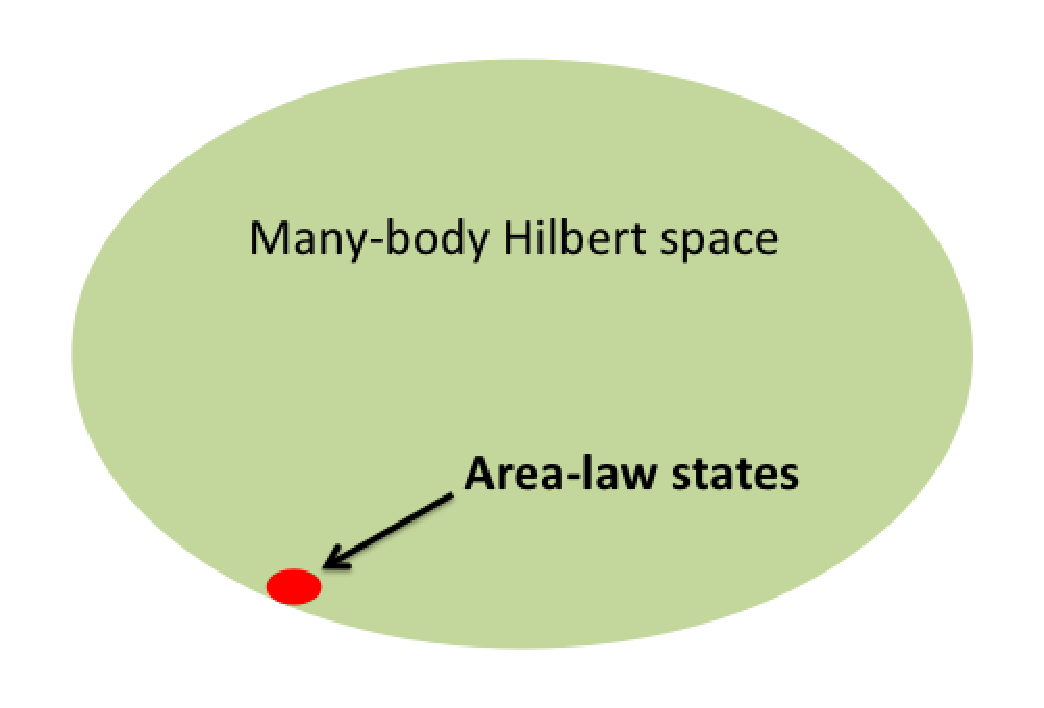
\includegraphics[width=0.9\textwidth]{orus-images/fig4.pdf}
            \end{figure}}
        \end{column}
\end{columns}   


\end{frame}

\begin{frame}{Why tensor networks?}
    \bi
    \item <1-> Tensor networks algorithms generalize renormalization group methods
    \bi
    \item <2-> Numerical RG (Wilson)
    \begin{figure}[htbp]
               \scalebox{0.6}{ %!TEX root = ../thesis.tex

\beginpgfgraphicnamed{mps1}
\begin{tikzpicture}[node distance=0.5cm]

\foreach \i in {1,2,3,4,5,6}
{
	\node[spin] (s\i) at (\i,0) {};
	\node[below of=s\i] {$H_\i$};
}

\foreach \i / \j in {1/2,2/3,3/4,4/5,5/6}
{
	\node[gamma] (g\i) at (\i+0.5,0.5*\i) {};
	\node[above left of=g\i] {$A_\i$};
%	\draw let \n1={\i+1} in (g\i) -- (s\n1);
	\draw (g\i) -- (s\j);
}

\foreach \i / \j in {2/1,3/2,4/3,5/4}
{
%	\draw let \n1={\i-1} in (g\i) -- (g\n1);
	\draw (g\i) -- (g\j);
}

\draw (s1) -- (g1);
\draw (g5) -- ($ (g5) + (0.5,0.5) $);

\end{tikzpicture}}
            \end{figure}
    \ei
    \item <3-> Interesting physical systems can be described by simple tensor networks
    \bi
    \item <4-> Including non-chiral topological or SPT order
    \ei
    \ei
\end{frame}

%%%%%%%%%%%%%%%%%%%%%%%%%%%%%%%%%%%%%%%%%
%%%%%%%%%% Outline code %%%%%%%%%%%%%%%%%
%%%%%%%%%%%%%%%%%%%%%%%%%%%%%%%%%%%%%%%%%
\section*{}
\begin{frame}
  \frametitle{Outline}
  \tableofcontents[section=1,hidesubsections]
\end{frame}

\AtBeginSection[]
{
  \frame<handout:0>
  {
    \frametitle{Outline}
    \tableofcontents[currentsection,hideallsubsections]
  }
}

\AtBeginSubsection[]
{
  \frame<handout:0>
  {
    \frametitle{Outline}
    \tableofcontents[sectionstyle=show/hide,subsectionstyle=show/shaded/hide]
  }
}
%%%%%%%%%%%%%%%%%%%%%%%%%%%%%%%%%%%%%%%%%
%%%%%%%%%% Content starts here %%%%%%%%%%
%%%%%%%%%%%%%%%%%%%%%%%%%%%%%%%%%%%%%%%%%



\section{What is a tensor network?}

\begin{frame}
  \frametitle{What is a tensor?}
 % \vskip-2cm
  \bi
  \only<1,3->{
  \item ... a state of many qubits $\ket{\psi} \in \bigotimes\limits_{i=1}^{N} \mathcal{H}_i$
  \note{Always have a 'computational basis'}
  \begin{figure}[t]
                %!TEX root = ../thesis.tex

%\beginpgfgraphicnamed{diagrams}
\begin{tikzpicture}[node distance=0.4cm]
%\tikzset{ellip/.style={ellipse (3 and 1), fill=blue!20, draw=black, inner sep=4pt}}
\tikzset{det/.style={circle=2pt,fill=blue!20,draw=black,inner sep=4pt}}
%\draw (1,1) ellipse [x radius=1cm,y radius=.5cm];
\node[ellipse, rotate=0, draw, fill=blue!20] (t) at (0,0) {\, \, $\psi$ \, \,};
\node (t1) at (-1.6, 0.6) {$i_1$};
\node (t2) at (-1.2 ,0.85) {$i_2$};
\node (t3) at (-0.8,1.1) {$i_3$};
\node (t4) at (-0.3,1.2) {$i_4$};
\node (t5) at (0.3, 1.2) {$i_5$};
\node (tN) at (1.6, 0.6) {$i_N$};
\node[rotate=-20] (d) at (0.6, 0.6) {...};
%\node (tl) at (1,-0.4) {$l$};
\draw[thick] (t1) -- (t);
\draw[thick] (t2) -- (t);
\draw[thick] (t3) -- (t);
\draw[thick] (t4) -- (t);
\draw[thick] (t5) -- (t);

\draw[thick] (tN) -- (t);
%\node[in of=t] {$\psi$};
\node (p) at (5,0) {$|\psi \rangle = \sum \psi_{i_1 i_2 ... i_N} \vert i_1 i_2 ... i_N \rangle$};


%\draw  (-0.8,2.4) node (v1) {} ellipse (1.2 and 0.4);
%\draw  (v1) ellipse (0 and 0);
\end{tikzpicture}
%\endpgfgraphicnamed
    \end{figure}}
  \only<2>{
  \item ... a map between Hilbert spaces
  \begin{figure}[t]
                \begin{tikzpicture}[node distance=0.4cm]]
\tikzset{det/.style={circle=2pt,fill=blue!20,draw=black,inner sep=4pt}}
\node[ellipse, rotate=0, draw, fill=blue!20] (t) at (0,0) {\, \, $\psi$ \, \,};
\node (t1) at (-1.6, 0.6) {$i_1$};
\node (t2) at (-1.2 ,0.85) {$i_2$};
\node (t3) at (-0.8,1.1) {$i_3$};
\node (o3) at (1.6, 0.6) {$o_3$};
\node (o2) at (1.2 ,0.85) {$o_2$};
\node (o1) at (0.8,1.1) {$o_1$};
\node[rotate=0] (d) at (0, 0.7) {...};

\begin{scope}[very thick,decoration={
    markings,
    mark=at position 0.5 with {\arrow{>}}}
    ] 
\draw[thick, postaction={decorate}] (t1) -- (t);
\draw[thick,postaction={decorate}] (t2) -- (t);
\draw[thick, postaction={decorate}] (t3) -- (t);
\draw[thick, postaction={decorate}] (t) -- (o1);
\draw[thick,postaction={decorate}] (t) -- (o2);
\draw[thick, postaction={decorate}] (t) -- (o3);
\end{scope}

\node (p) at (4.5,0) {$\ket{\psi} = \sum \psi_{i_1 i_2 .. o_1 o_2 ..} \vert o_1 o_2 .. \rangle \langle i_1 i_2 .. \vert$};

\end{tikzpicture}
    \end{figure}}
  \only<3>{
  \item with which we can form contractions
  \note{using any subset of the legs}
  \begin{figure}[t]
        \begin{tikzpicture}[node distance=0.4cm]]


\tikzset{det/.style={circle=2pt,fill=blue!20,draw=black,inner sep=4pt}}
\node[ellipse, rotate=0, draw, fill=blue!20] (t) at (0,0) {\, \, $\psi$ \, \,};
\node (t1) at (-1.6, 0.6) {$i_1$};
\node (t2) at (-1.2 ,0.85) {$i_2$};
\node (t3) at (-0.8,1.1) {$i_3$};
\node (o3) at (1.6, 0.6) {};
\node (o2) at (1.2 ,0.85) {};
\node (o1) at (0.8,1.1) {};
\node[rotate=0] (d) at (0, 0.7) {...};

\begin{scope}[very thick,decoration={
    markings,
    mark=at position 0.5 with {\arrow{>}}}
    ] 
\draw[thick, postaction={decorate}] (t1) -- (t);
\draw[thick,postaction={decorate}] (t2) -- (t);
\draw[thick, postaction={decorate}] (t3) -- (t);
\draw[thick, postaction={decorate}] (t) -- (o1.center);
\draw[thick,postaction={decorate}] (t) -- (o2.center);
\draw[thick, postaction={decorate}] (t) -- (o3.center);
\end{scope}


\node[ellipse, rotate=0, draw, fill=blue!20] (rt) at (4,0) {\, \, $\varphi$ \, \,};
\node (rt1) at (2.4, 0.6) {};
\node (rt2) at (2.8 ,0.85) {};
\node (rt3) at (3.2,1.1) {};
\node (ro3) at (5.6, 0.6) {$o_3$};
\node (ro2) at (5.2 ,0.85) {$o_2$};
\node (ro1) at (4.8,1.1) {$o_1$};
\node[rotate=0] (d) at (4, 0.7) {...};

\begin{scope}[very thick,decoration={
    markings,
    mark=at position 0.5 with {\arrow{>}}}
    ] 
\draw[thick, postaction={decorate}] (rt1.center) -- (rt);
\draw[thick,postaction={decorate}] (rt2.center) -- (rt);
\draw[thick, postaction={decorate}] (rt3.center) -- (rt);
\draw[thick, postaction={decorate}] (rt) -- (ro1);
\draw[thick,postaction={decorate}] (rt) -- (ro2);
\draw[thick, postaction={decorate}] (rt) -- (ro3);

\draw[thick] (o3.center) to [bend left=5] node[below] {} (rt1.center);
\draw[thick] (o2.center) to [bend left=15] node[below] {} (rt2.center);
\draw[thick] (o1.center) to [bend left=30] node[below] {} (rt3.center);
\end{scope}
\end{tikzpicture}
    \end{figure}
  }
  \only<4>{
  \item or decompose using SVD.
  \begin{figure}
  \centering
   %!TEX root = ../thesis.tex

\begin{tikzpicture}

\node[det] (Ap) at (0,-0.5) {$A$};
% \node[det] (Bp) at (2,-0.5) {$B$};
% \node[det] (Cp) at (1,-2) {$C$};

% \draw[thick] (Ap.north east) -- (Bp.north west);
% \draw[thick] (Ap.south east) -- (Bp.south west);
% \draw[thick] (Ap.south) -- (Cp.north west);
% \draw[thick] (Bp.south) -- (Cp.north east);

\draw[thick] (Ap.north west) -- node[above] {$i$} +(-0.5,0.5);
\draw[thick] (Ap.south west) -- node[below] {$j$} +(-0.5,-0.5);
\draw[thick] (Ap.north east) -- node[above] {$k$} +(0.5,0.5);
\draw[thick] (Ap.south east) -- node[below] {$l$} +(0.5,-0.5);

% \draw[thick] (Cp.south) -- node[right] {$k$} +(0,-0.5);
% \draw[thick] (Bp.east) -- node[below] {$l$} +(0.5,0);

% next panel

\node[det] (U) at (4,-0.5) {$U$};
\node[det] (V) at (6,-0.5) {$V$};
\node[lambda] (S) at (5,-0.5) {};
\node[above of=S,node distance=0.3cm] {$S$};

\draw[thick] (U) -- (S) -- (V);

\draw[thick] (U.north west) -- node[above] {$i$} +(-0.5,0.5);
\draw[thick] (U.south west) -- node[below] {$j$} +(-0.5,-0.5);
\draw[thick] (V.south east) -- node[right] {$l$} +(0.5,-0.5);
\draw[thick] (V.north east) -- node[right] {$k$} +(0.5,0.5);

\end{tikzpicture}

  \end{figure}
  }
  \ei
\end{frame}
\begin{frame}
  \only<1>{
  \frametitle{What is a tensor network?}}
  \only<2->{
  \frametitle{What is a tensor network {\em state}?}}
  \bi
  \item ... a contraction scheme for building tensors
  \begin{figure}[t]
                \begin{tikzpicture}[node distance=0.4cm]

\node[det] (t) at (-1,-3.8) {$A$};
\node[det] (q) at (1,-3.8) {$B$};
\node (ti) at (-2,-3.8) {$i$};
\node (qn) at (2,-3.4) {$n$};
\node (qr) at (2,-4.2) {$r$};
\draw[thick] (ti) -- (t);
\draw[thick] (q) -- (qn);
\draw[thick] (q) -- (qr);
\draw[thick] (t) to [bend right=30] node[below] {$k$} (q);
\draw[thick] (t) to [bend left=30] node[above] {$j$} (q);
%\node[below of=q] {$q$};
%\node[below of=t] {$t$};
\node at (5,-3.8) {$\sum_{jk} A_{ijk} B_{jknr}$};

\end{tikzpicture}
    \end{figure}
  \pause
  \item ... an ansatz for wavefunctions using a tensor network
  \begin{figure}[t]
                \begin{tikzpicture}[node distance=0.4cm]
\tikzset{gamma/.style={circle=2pt,draw=black!100, very thick, fill=blue!40, inner sep=3pt}}


\begin{scope}[decoration={
    markings,
    mark=at position 0.5 with {\arrow{>}}}
    ]

\foreach \i in {1,...,6} {
	\node[gamma] (G\i) at (1.5*\i,0) {$A$};
	\node (l\i) at ($ (G\i) + (0, 1) $) {$$};
	\draw[very thick, red!100, postaction={decorate}] (G\i) -- (l\i);
	%\node[below of=G\i] {$A$};
}

\foreach \i in {7} {
	\node[] (G\i) at (1.5*\i,0) {$...$};
    }  
    
\foreach \i / \j in {1/2,2/3,3/4,4/5,5/6, 6/7} {
	\draw[very thick, postaction={decorate}] (G\j) -- (G\i);
}
\node (b0) at (0, 0) {$...$};
\draw[very thick, postaction={decorate}] (G1) -- (b0);

\end{scope}
\end{tikzpicture}

        \caption{Matrix Product State ansatz}
    \end{figure}
    \note{contraction scheme is one tensor per site}
   \note{Reason for title matrix product state: each w.f. coefficient is computed
         using a product of matrices}
   \note{Goal is to find a local computational procedure for specifying coefficients of         the wavefunction}
   \note{Similar but not quite equivalent to specifying a circuit of local quantum gates          to construct the state}
  \note{number of parameters linear in system size, fixed bond dimension}
  \note{bond dimension may need to go up to improve wavefunction accuracy}
  \note{given such a procedure, we automatically satisfy entanglement bounds}
   \note{In order for this to not be every wavefunction, have to fix bond dimension}
  \ei
\end{frame}
\begin{frame}
  \frametitle{What is a tensor network {\em state}?}
  \bi
  \item ... with internal bond dimension $M$ fixed.
  \begin{figure}[t]
    \raggedright
    \begin{tikzpicture}
\foreach \i in {1,...,3}
\foreach \j in {2}
{ {
	\node (G\i\j) at (1.5*\i+1*\j,1.5*\j) {};
} }

\foreach \i in {2}
\foreach \j in {1, 3}
{ {
	\node (G\i\j) at (1.5*\i+1*\j,1.5*\j) {};
} }

\foreach \k / \i in {1/2}
\foreach \l / \j in {1/2}
{ {
	\node at (G\i\j) [peps] {};
	\draw[thick] (G\i\j) -- node[below right ] {$d$} +(0,-1);
	\node at ($ (G\i\j)+(0,-1.3) $) {$\phi_i$};
} }
\foreach \i in {2}
\foreach \j / \l in {1/2,2/3}
{ {
	\draw[thick] (G\i\j) -- node[left] {$M$} (G\i\l);
	\draw[thick] (G\j\i) -- node[above] {$M$} (G\l\i);
} }

\foreach \i in {1,...,4}
\foreach \j in {1,...,4}
{ {
	\node (G\i\j) at (2.5+1.2*\i+0.8*\j,1*\j) [inv] {};
} }

\foreach \i / \j / \k in {2/2/1,2/3/2,2/4/3,3/2/4,3/3/5,3/4/6,4/2/7,4/3/8,4/4/9}
{
	\node at (G\i\j) [peps] {};
	\draw[thick] (G\i\j) -- node[below] {$p_{\k}$} +(0,-0.5);
}
\foreach \i in {2,3,4}
\foreach \j / \l in {2/3,3/4}
{ {
	\draw[thick] (G\i\j) -- (G\i\l);
	\draw[thick] (G\j\i) -- (G\l\i);
} }
\end{tikzpicture}
    \end{figure}
    
    \item With no bounds on $M$, anything is possible:
    \begin{figure}[t]
    \raggedright
    \begin{tikzpicture}[node distance=0.4cm]

\foreach \i / \j in {1/A,2/B,3/A,4/B,5/A}
{
	\node[gamma] (G\i) at (2*\i-2,2.5) {};
	\node[below of=G\i] {$U^\i$};
	\draw[thick] (G\i) -- ($ (G\i) + (0, 0.75) $);
}
\foreach \i / \j in {1/A, 2/B,3/A,4/B}
{
	\node[lambda] (l\i) at (2*\i-1,2.5) {};
	\node[below of=l\i] {$\lambda^\i$};
}

\foreach \i / \j in {1/2,2/3,3/4,4/5}
{
	\draw[thick] (l\i) -- (G\i);
	\draw[thick] (l\i) -- (G\j);
}

%\draw[thick,dashed] (l1) -- ($ (l1) + (-0.5,0) $);
%\draw[thick,dashed] (l6) -- ($ (l6) + (0.5,0) $);

\end{tikzpicture}
    \end{figure}
  \ei
\end{frame}
\begin{frame}{Working with tensor network states}
%\framesubtitle{Entanglement}
\bi 
\item Rank of reduced density matrix (and entanglement entropy) bounded by total bond dimension
\begin{figure}
\raggedright
\begin{tikzpicture}[node distance=0.6cm]
\node[side] (kL) at (0,0) {$\psi_L$};
\node[side] (kR) at (1.3, 0) {$\psi_R$};
\draw[thick] (kL) -- node[below] {$i$} (kR);
\node (kLp) at (0, 1) {};
\draw[thick] (kL) -- node[left] {$p$} (kLp);

\node[side] (bL) at (0,-1) {$\psi_L^*$};
\node[side] (bR) at (1.3, -1) {$\psi_R^*$};
\draw[thick] (bL) -- node[above] {$j$} (bR);
\node (bLp) at (0, -2) {};
\draw[thick] (bL) -- node[left] {$p'$} (bLp);

\node (kRp) at ($(kR.north)+(0.4, 0.4)$) {};
\node (bRp) at ($(bR.south)+(0.4, -0.4)$) {};
\draw[thick] (kR.north) to [bend left= 90] (kRp.center) to  [bend left=90] node[right] {$q$}  (bRp.center) to [bend left=90] (bR.south);


% \node[side] (UL) at (4, 0) {$U_S$};
% \node[side] (VL) at (5.4, 0) {$V_S$};
% \node[lambda] (SL) at (4.7, 0) {};
% \node[bel0w of=S] {$S_S$};

% \draw[thick] (UL) -- (SL) -- (VL);
% \node[side] (kL) at (4,0) {$\psi_S$};
% \node[side] (kR) at (7, 0) {$\psi_E$};
% \draw[thick] (VL) -- node[below] {$i$} (kR);
% \node (kLp) at (4, 1) {};
% \draw[thick] (UL) -- node[left] {$p_S$} (kLp);


% \node[side] (UdL) at (4, -1) {$U_S^*$};
% \node[side] (VdL) at (5.4, -1) {$V_S^*$};
% \node[lambda] (SdL) at (4.7, -1) {};
% \node[above of=SdL] {$S_S$};

% \draw[thick] (UdL) -- (SdL) -- (VdL);
% \node[side] (bR) at (7, -1) {$\psi_E^*$};
% \draw[thick] (VdL) -- node[above] {$j$} (bR);
% \node (bLp) at (4, -2) {};
% \draw[thick] (UdL) -- node[left] {$p'_S$} (bLp);

% \node (kRp) at ($(kR.north)+(0.4, 0.4)$) {};
% \node (bRp) at ($(bR.south)+(0.4, -0.4)$) {};
% \draw[thick] (kR.north) to [bend left= 90] (kRp.center) to  [bend left=90] node[right] {$p_E$}  (bRp.center) to [bend left=90] (bR.south);


\end{tikzpicture}
\end{figure}
\note{\psi_s can be thought of as a map from edge to physical space, but its not isometric (rectangle unitary)}
\note{ image psi_S is still an interesting set though}
\item Spectrum can be computed without using $U_S$
\item $U_S$ columns are orthogonal Schmidt states
$$
\ket{\psi} = \sum\limits_k U_S^{k p_s} \ket{p_s} \Lambda_k \ket{p_E} U_E^{k p_e}
$$
\ei 
\end{frame}
\begin{frame}{Working with tensor network states}
%\framesubtitle{Entanglement}
\bi 
\item Computing correlation functions in infinite MPS
\ei 
\begin{figure}[t]
\centering
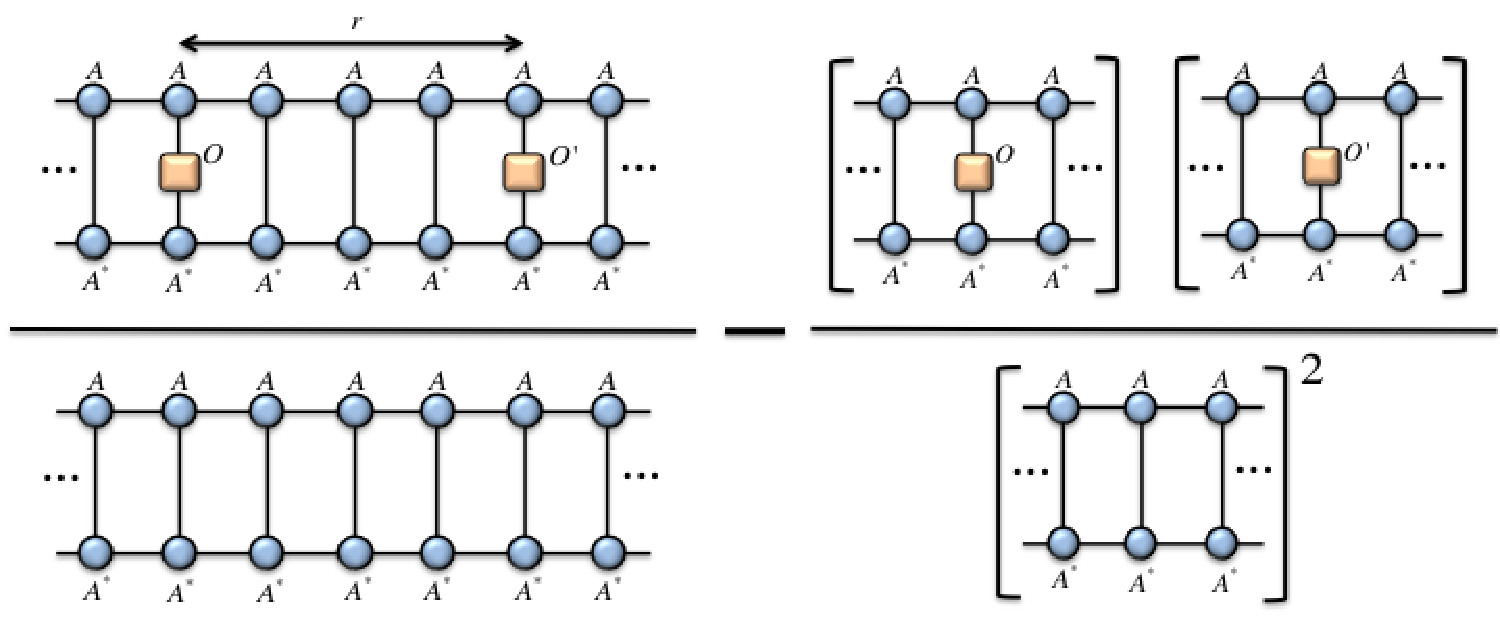
\includegraphics[width=\textwidth]{orus-images/fig13}
%\begin{tikzpicture}[node distance=0.5cm]

\foreach \i in {1,...,5} {
	\node (Gp\i) at (1.5*\i,-2.5) [gamma] {};
	\node (Gpp\i) at ($ (Gp\i) + (0,-1) $) [gamma] {};
	\draw[thick] (Gp\i) -- (Gpp\i);
	\node[above of=Gp\i] {$A^\i$};
	\node[below of=Gpp\i] {$(A^\i)^*$};
}
\foreach \i / \j in {1/2,2/3,3/4,4/5} {
	\draw[thick] (Gp\i) -- (Gp\j);
	\draw[thick] (Gpp\i) -- (Gpp\j);
}

\foreach \i in {1,...,5} {
	\node (Gp\i) at (1.5*\i,-5.5) [gamma] {};
	\node (Gpp\i) at ($ (Gp\i) + (0,-2) $) [gamma] {};
	\node (O\i) at ($ (Gp\i) + (-0,-1) $) [operator] {};
	
	\draw[thick] (Gp\i) -- (O\i);
	\draw[thick] (Gpp\i) -- (O\i);
	
	\node[above of=Gp\i] {$A^\i$};
	\node[below of=Gpp\i] {$(A^\i)^*$};
	\node[above left of=O\i] {$W^\i$};
}
\foreach \i / \j in {1/2,2/3,3/4,4/5} {
	\draw[thick] (Gp\i) -- (Gp\j);
	\draw[thick] (Gpp\i) -- (Gpp\j);
	\draw[thick] (O\i) -- (O\j);
}

\end{tikzpicture}

\caption{Diagram for $C(r) = \ev{O_i O'_{i+r}}- \ev{O_i}\ev{O'_{i+r}}$}
\end{figure}
\bi 
\item  $\ev{O_i O'_{i+r}} = \vbraopket{v_L}{T_O T_I^r T_{O'}}{v_R}$
\ei 
\end{frame}

\section{AKLT: the canonical MPS}
\begin{frame}{Symmetry and MPS}

MPS representations are {\em gauge equivalent} if 
\begin{figure}
\centering
\begin{tikzpicture}
\begin{scope}[very thick,decoration={
    markings,
    mark=at position 0.5 with {\arrow{>}}}
    ] 

\node[peps] (A1) at (-4.1, 0) {};
\node (li) at ($(A1) + (-1, 0) $) {};
\draw[thick, postaction={decorate}] (li.center) -- (A1.west);
\draw[thick, postaction={decorate}] (A1.east) -- node[right] {} +(1,0);
\draw[thick, postaction={decorate}] (A1.north) -- node[above] {} +(0,0.5);

\node at (-2.3, 0.5){$= e^{i \theta}$};    

\node[peps] (A) at (0, 0) {};
\node[draw] (Ul) at ($(A) + (-1, 0) $) {$U$};
\node[draw] (Ur) at ($(A) + (1, 0) $) {$U^{\dagger}$};
\node (LI) at ($(Ul) + (-1, 0) $) {};
\draw[thick, postaction={decorate}] (LI.center) -- (Ul.west);
\draw[thick, postaction={decorate}] (Ur.east) -- node[right] {} +(0.5,0);
\draw[thick, postaction={decorate}] (Ul) -- (A);
\draw[thick, postaction={decorate}] (A) -- (Ur);
\draw[thick, postaction={decorate}] (A.north) -- node[above] {} +(0,0.5);

\end{scope}
\end{tikzpicture}
\end{figure}

\begin{theorem}
Two (simple) MPS specify the same state if and only if they have a gauge equivalence between them.
\end{theorem}
Therefore symmetric MPS can be represented using a symmetric site tensor.
\begin{figure}
\centering
\begin{tikzpicture}
\begin{scope}[very thick,decoration={
    markings,
    mark=at position 0.5 with {\arrow{>}}}
    ] 

\node[peps] (A1) at (-4.1, 0) {};
\node (li) at ($(A1) + (-1, 0) $) {};
\draw[thick, postaction={decorate}] (li.center) -- (A1.west);
\draw[thick, postaction={decorate}] (A1.east) -- node[right] {} +(1,0);
\draw[thick, postaction={decorate}] (A1.north) -- node[above] {} +(0,0.5);

\node at (-2.3, 0.5){$= e^{i \theta_g}$};    

\node[peps] (A) at (0, 0) {};
\node[draw] (Up) at ($(A) + (0, 1) $) {$U_g$};
\node[draw] (Ul) at ($(A) + (-1, 0) $) {$V_g$};
\node[draw] (Ur) at ($(A) + (1, 0) $) {$V_g^{\dagger}$};
\draw[thick, postaction={decorate}] (Up.north) -- node[above] {} +(0,0.5);
\node (LI) at ($(Ul) + (-1, 0) $) {};
\draw[thick, postaction={decorate}] (LI.center) -- (Ul.west);
\draw[thick, postaction={decorate}] (Ur.east) -- node[right] {} +(0.5,0);
\draw[thick, postaction={decorate}] (A) -- (Up);
\draw[thick, postaction={decorate}] (Ul) -- (A);
\draw[thick, postaction={decorate}] (A) -- (Ur);

\end{scope}
\end{tikzpicture}
\end{figure}

\end{frame}
\begin{frame}{AKLT: the canonical MPS}
\begin{figure}
\centering
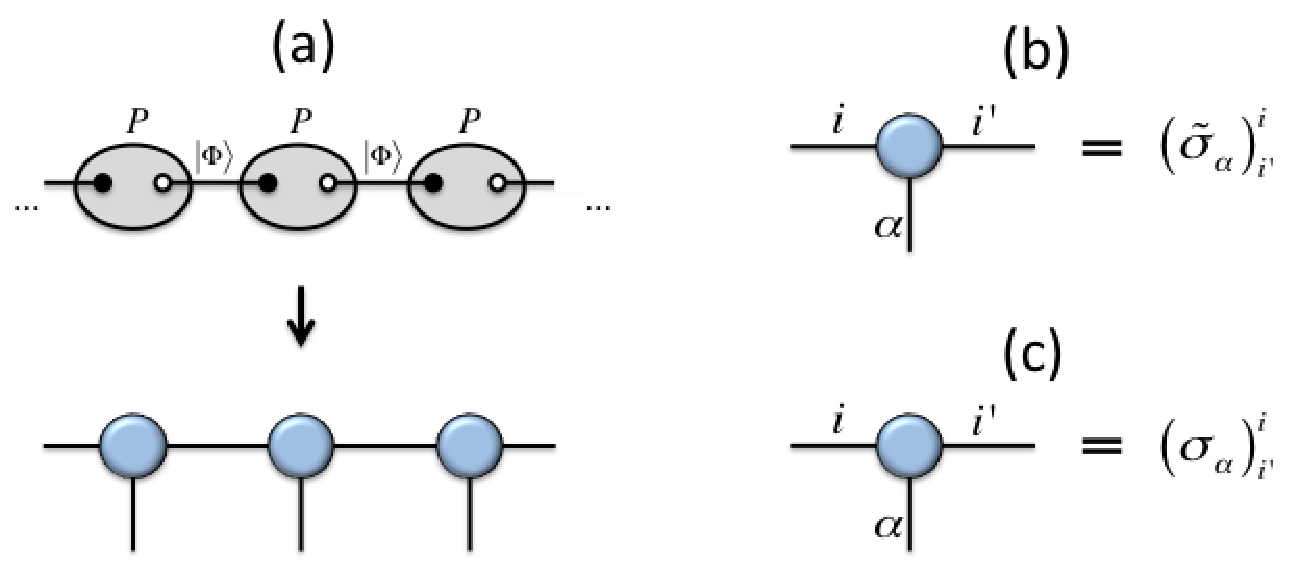
\includegraphics[width=\textwidth]{orus-images/fig22}
\caption{Derivation of the site tensors for the AKLT state}
\end{figure}
\end{frame}
\begin{frame}{AKLT: Results}
\bi 
\item Transfer matrix is simple (one eigenvalue of magnitude $1$).
\item Correlations decay with power $-\frac{1}{3}$
\item Reduced density matrix has eigenvalues $\frac12, \frac12$
\item Can't continuously tune to a product state without breaking SU(2) symmetry
\item Two Schmidt states look like infinite system ground state far from boundary
\item Schmidt states differ by a spin 1/2 degree of freedom living near boundary
\item Degeneracy 2 on half-infinite chain, 1 on circle
\item Advanced result: Can't continuously tune to a product state without breaking $D_2$ AND time-reversal AND spatial reflection symmetry
\ei 
\end{frame}

\section{Constructing the toric code state}
\begin{frame}
 \frametitle{Nuts and bolts}
\begin{itemize}

%\only<1,3->{\vskip-1cm}

\only<1-4>{
\item<1-> GHZ-state
\begin{figure}[t]
\raggedright

\begin{tikzpicture}[node distance=0.2cm]

\node[GHZ] (G) at (0, 0) {};
\foreach \i in {1, 2, 3}
  {
 \pgfmathsetmacro{\ang}{120*\i}
 \pgfmathsetmacro{\x}{cos(\ang)}
 \pgfmathsetmacro{\y}{sin(\ang)}
 \node (g\i) at ($ (G)+(0.8*\x, 0.8*\y) $) {};
  \draw[thick] (G) -- (g\i);
 }

 
 
 \node at (3, 0) {$\ket{GHZ} = \ket{000}+\ket{111}$};

 
\end{tikzpicture}
\end{figure}

\only<2>{
\bi
\item $\mathbf{Z}_2$ symmetric
\ei
\begin{figure}[t]
\begin{tikzpicture}[node distance=0.2cm]

\node[GHZ] (G) at (0, -2) {};
\foreach \i in {1, 2, 3}
  {
 \pgfmathsetmacro{\ang}{120*\i}
 \pgfmathsetmacro{\x}{cos(\ang)}
 \pgfmathsetmacro{\y}{sin(\ang)}
 \node[draw, rotate=\ang] (gx\i) at ($ (G)+(0.6*\x, 0.6*\y) $) {$X$};
 \node[inv] (g\i) at ($ (G)+(1.5*\x, 1.5*\y) $) {};
 }
 
\foreach \i in {1, 2, 3}
  {
 \draw[thick] (G) -- (gx\i) --(g\i);
 } 
 
\node at (1.8, -2) {$=$};

\node[GHZ] (G3) at (2.4, -2) {};
\foreach \i in {1, 2, 3}
  {
 \pgfmathsetmacro{\ang}{120*\i}
 \pgfmathsetmacro{\x}{cos(\ang)}
 \pgfmathsetmacro{\y}{sin(\ang)}
 \node (g\i) at ($ (G3)+(0.8*\x, 0.8*\y) $) {};
 }
 \foreach \i in {1, 2, 3}
  {
 \draw[thick] (G3) -- (g\i);
 }

\end{tikzpicture}
\end{figure}
}

\only<3>{
\bi
\item Contracting gives larger GHZ state
\ei
\begin{figure}[t]
\begin{tikzpicture}[node distance=0.2cm]

\node[GHZ] (G) at (0, 0) {};
\foreach \i in {1, 2, 3}
  {
 \pgfmathsetmacro{\ang}{120*\i}
 \pgfmathsetmacro{\x}{cos(\ang)}
 \pgfmathsetmacro{\y}{sin(\ang)}
 \node[inv] (g\i) at ($ (G)+(0.8*\x, 0.8*\y) $) {};
 }
 
\foreach \i in {1, 2, 3}
  {
 \draw[thick] (G) --(g\i);
 } 
 


\node[GHZ] (G2) at (1, 0) {};
\foreach \i in {1, 2, 3}
  {
 \pgfmathsetmacro{\ang}{180+120*\i}
 \pgfmathsetmacro{\x}{cos(\ang)}
 \pgfmathsetmacro{\y}{sin(\ang)}
 \node (g2\i) at ($ (G2)+(0.8*\x, 0.8*\y) $) {};
 }
 \foreach \i in {1, 2, 3}
  {
 \draw[thick] (G2) -- (g2\i);
 }
 
 \draw[thick] (G) -- (G2);
 
 \node at (2, 0) {$=$};

\node[GHZ] (G) at (3, 0) {};
\foreach \i in {1, 2, 3, 4}
  {
 \pgfmathsetmacro{\ang}{45+90*\i}
 \pgfmathsetmacro{\x}{cos(\ang)}
 \pgfmathsetmacro{\y}{sin(\ang)}
 \node[inv] (g\i) at ($ (G)+(\x, \y) $) {};
 }
 
\foreach \i in {1, 2, 3, 4}
  {
 \draw[thick] (G) --(g\i);
 } 
 

\end{tikzpicture}
\end{figure}
}
}

\only<4->{
\item GHZ-state in basis of $X$
\note{Same properties as GHZ}
\begin{figure}[t]
\raggedright

\begin{tikzpicture}[node distance=0.2cm]

\node[circlewc] (G) at (0, 0) {};
\foreach \i in {0, 1, 2}
  {
 \pgfmathsetmacro{\ang}{90*\i}
 \pgfmathsetmacro{\x}{cos(\ang)}
 \pgfmathsetmacro{\y}{sin(\ang)}
 \node (g\i) at ($ (G)+(0.8*\x, 0.8*\y) $) {};
  \draw[thick] (G) -- (g\i);
 }
 
 
 \node at (4, 0) {$\ket{X} = \ket{000}+\ket{011}+ \ket{101} + \ket{110}$};

 
\end{tikzpicture}

\end{figure}
}

\only<5->{
\item<5-> C-NOT Gate
\begin{figure}[t]
\raggedright

\begin{tikzpicture}[node distance=0.2cm]

\node[GHZ] (G) at (0, 0) {};
\foreach \i in {0, 2}
  {
 \pgfmathsetmacro{\ang}{90*\i}
 \pgfmathsetmacro{\x}{cos(\ang)}
 \pgfmathsetmacro{\y}{sin(\ang)}
 \node (g\i) at ($ (G)+(0.8*\x, 0.8*\y) $) {};
  \draw[thick] (G) -- (g\i);
 }

\node[circlewc] (X) at (0, -1) {};
\foreach \i in {0, 2}
  {
 \pgfmathsetmacro{\ang}{90*\i}
 \pgfmathsetmacro{\x}{cos(\ang)}
 \pgfmathsetmacro{\y}{sin(\ang)}
 \node (x\i) at ($ (X)+(0.8*\x, 0.8*\y) $) {};
  \draw[thick] (X) -- (x\i);
 }
 
 \draw[thick] (G) -- (X);

 
\end{tikzpicture}

\end{figure}

\item<6-> GHZ can be used to synchronize many operators: C-NOT-NOT-NOT-NOT
\item<7-> Using GHZ as the MPS site tensor creates a CAT state
}
 \end{itemize}
 \end{frame}

\begin{frame}{Toric Code State}
\begin{figure}
\centering
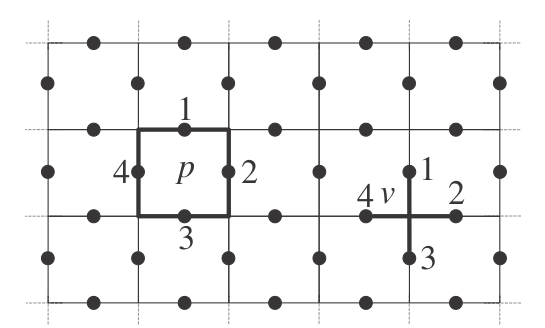
\includegraphics[width=\textwidth]{diagrams/WUl3V.png}
\caption{Toric code}
\end{figure}
\end{frame}
\begin{frame}{Toric Code}
$$
H = -J_a \sum_s A_s - J_b \sum_p B_p \ , 
$$
where $A_v$ and $B_p$ are vertex and plaquette operators such that 
$$
A_v = \prod_{i \in v} \sigma_z^i   \ , \ \ \ \ \ \  B_p = \prod_{i \in p} \sigma_x^{i} \ . 
$$

$$
\ket{\Psi_{TC}} =  \prod_{v} \frac{\left( \mathbb{I} + A_v\right)}{2} \prod_{p} \frac{\left( \mathbb{I} + B_p\right)}{2}\ket{00..} =  \prod_{p} \frac{\left( \mathbb{I} + B_p \right)}{2} \ket{00..} \ ,
$$

$\ket{\Psi_{TC}}$ is a equal weighted superpositions of all 'loops', where loops indicate positions of $\ket{1}$
\end{frame}
\begin{frame}{Toric Code Site Tensors}
\bi 
\item $\mathbb{I} + B_p$ is just a C-NOT-NOT-NOT-NOT
\item To get a toric code PEPS, just apply this operator on all plaquettes to product state $\ket{00..}$
\begin{figure}
\centering
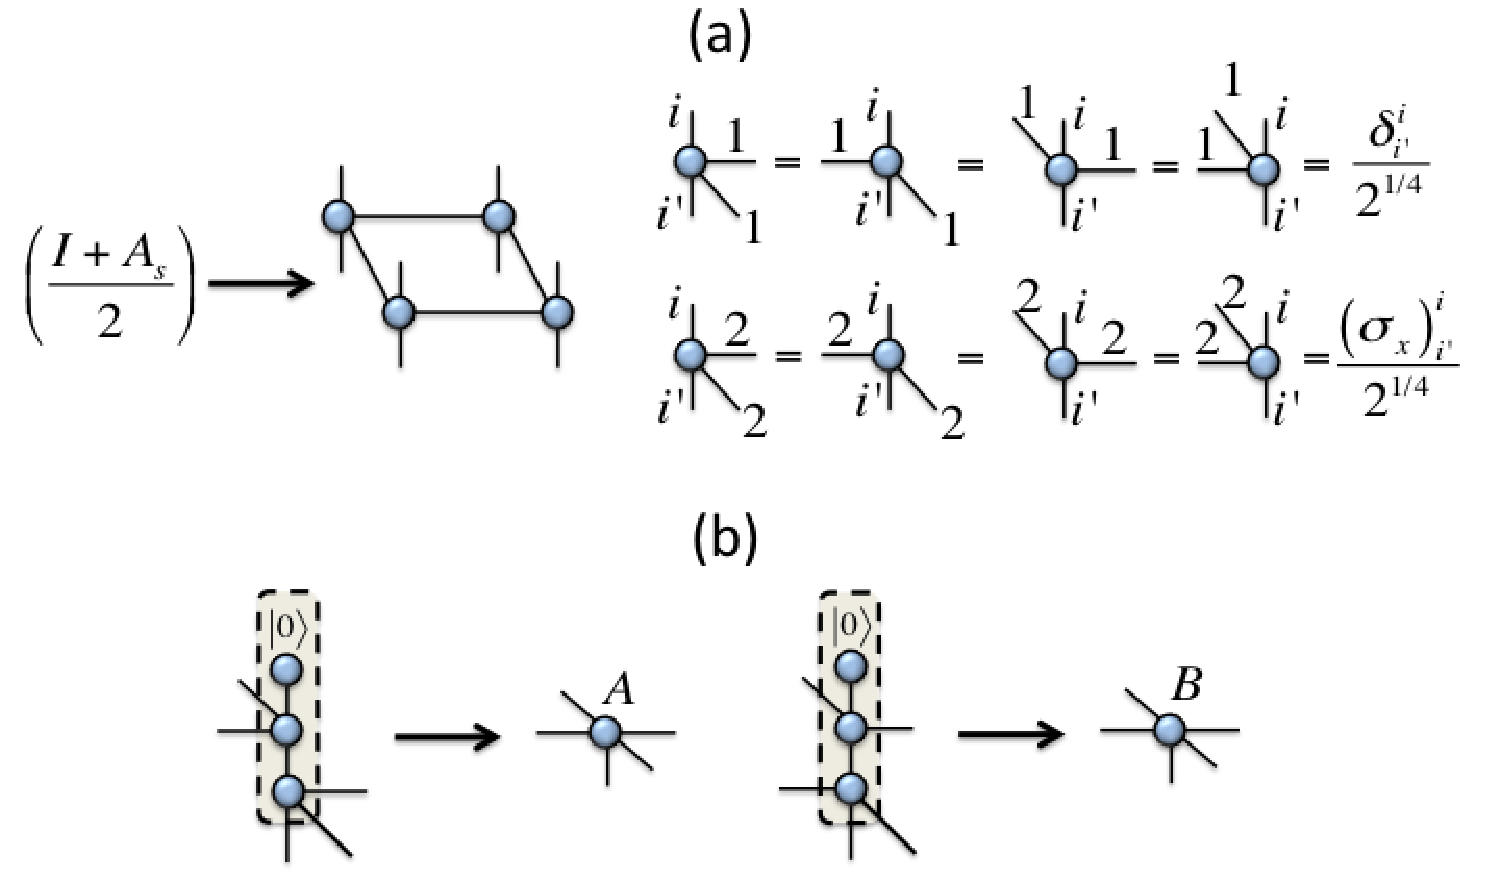
\includegraphics[width=0.8\textwidth]{orus-images/fig29.pdf}
\end{figure}
\ei
\end{frame}
\begin{frame}{Toric Code Results}
\vskip-1cm
\begin{figure}
\raggedright
\begin{tikzpicture}
\foreach \i in {1,...,4}
\foreach \j in {1,...,4}
{ {
	\node (G\i\j) at (2.5+1.2*\i+0.8*\j,1*\j) [inv] {};
} }

\foreach \i / \j / \k in {2/2/1,2/3/2,2/4/3,3/2/4,3/3/5,3/4/6,4/2/7,4/3/8,4/4/9}
{
	\node at (G\i\j) [circlewc] {};
	%\draw[thick] (G\i\j) -- node[below] {$p_{\k}$} +(0,-0.5);
}
\foreach \i / \j / \k in {2/2/1,2/3/2,2/4/3,3/2/4,3/3/5,3/4/6}
{
	\node (HR\i\j) at ($(G\i\j)+(0.6, 0)$) [GHZ] {};
	\node (HU\j\i) at ($(G\j\i)+(0.4, 0.5)$) [GHZ] {};
	\draw[thick] (HR\i\j) -- node[above] {} +(0,0.3);
	\draw[thick] (HU\j\i) -- node[above] {} +(0,0.3);
}
\foreach \i in {2,3,4}
\foreach \j / \l in {2/3,3/4}
{ {
	\draw[thick] (G\i\j) -- (G\i\l);
	\draw[thick] (G\j\i) -- (G\l\i);
} }
\end{tikzpicture}
\end{figure}
\vskip-1cm
\bi 
\item Topological order signified by virtual level symmetry
\item Around a trivial cycle, virtual symmetry leads to correction to entanglement area law. 
\item Around a nontrivial cycle, virtual symmetry maps to degenerate ground states
\item This is generic for non-chiral topological order
\ei 
\end{frame}

\section*{}

\frame{
  \vspace{2cm}
  {\huge Questions?}

  \vspace{3cm}
  \begin{flushright}
    Brayden Ware

    \structure{\footnotesize{brayden@physics.ucsb.edu}}
  \end{flushright}
}

\frame{
  \vfill
  \centering
  \highlighton{
  \usebeamerfont*{frametitle}Bonus slides

  %\usebeamerfont*{framesubtitle}Bonus slides
  }
  \vfill
}

\begin{frame}
  \frametitle{Resources}
  \vskip-1.7cm
  %\framesubtitle{If you want to improve this style}
  \bibliography{references}
  %\beamertemplatearticlebibitems
\end{frame}



\end{document}
